\chapter{Proposed solutions} \label{ch:proposed_solutions}

In this thesis, we use deep learning-based methods to solve the problem of long term person re-identification. We propose three approaches: Edge-based method, Skeleton-based method, and Combined method. In all of these methods, the first step is the preprocessing of the video sequences. As each video consists of a sequence of images, we describe the preprocessing on individual image frames. The outputs of the preprocessing phase are then fed into a neural network. For the model implementation, we use the Keras library. 

\section{Edge-based method}

In the Edge-based method, the preprocessing phase consists of a transformation of the original video frames into gray-scale images depicting the edges from the original images. We use this approach to remove information about a person's clothing, which typically changes in the long-term scope. The model is therefore forced to use information about the movement and body shape of the persons to perform the re-id. The transformed videos are then fed into a neural network. 

\subsection{Edge extraction}
For the video frames transformation in the preprocessing phase of this method, we use the edge detection neural network described in  \ref{tb:edge_detection}. An example of this transformation applied on one video frame from the MARS dataset \cite{MARS} is depicted in figure \ref{fig:countour_extraction}.

\begin{figure}[h!]
    \centering
    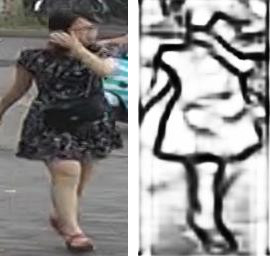
\includegraphics[scale=0.4]{figures/contours_example.jpg}
    \caption{Edge extraction example: left hand side - original image, right hand side - image after edge extraction}
    \label{fig:countour_extraction}
\end{figure}

\subsection{Neural Network description}
The structure of the neural network used in the edge-based model is illustrated in Figure \ref{fig:nnModel}. 

The first part of this neural network consists of three ConvLSTM layers (see Section \ref{tb:convLstm}), each of them followed by a batch normalization layer \cite{batch_normalization}. The input to the first ConvLSTM layer is a sequence of 20 images with the resolution of 64$\times$64 pixels. In the last ConvLSTM layer, this sequence is combined into one output, which is then fed into the second part of this network. 

The second part of the network consists of an 2D Average Pooling layer, followed by a Flatten layer and two Dense layers with ReLu and Softmax activation functions.

\begin{figure}[h!]
    \centering
    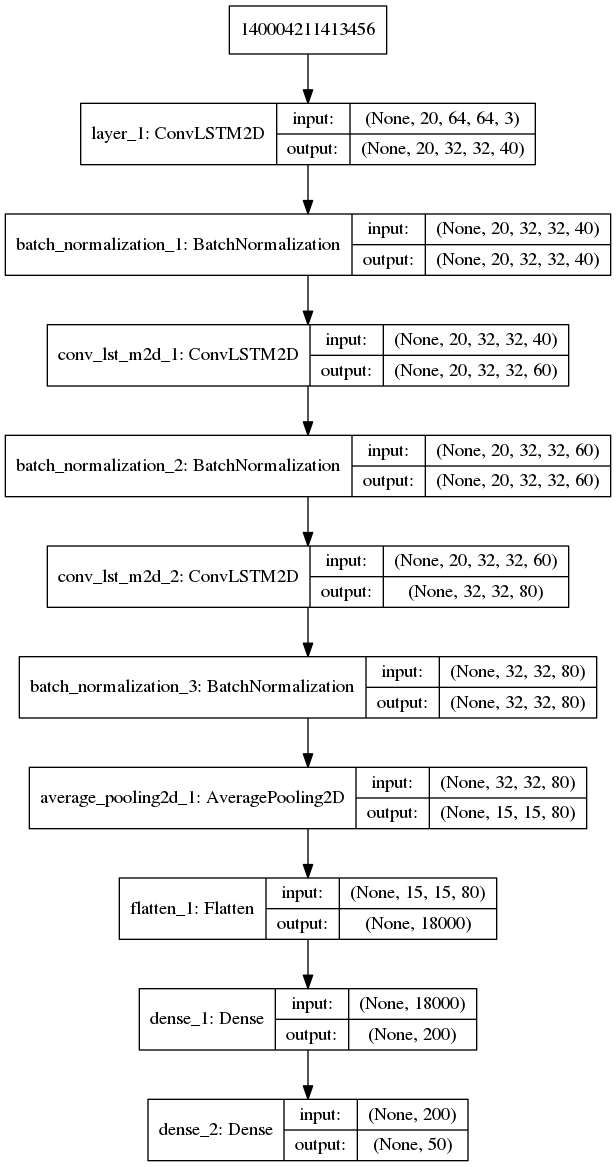
\includegraphics[scale=0.4]{figures/model.png}
    \caption{Edge based model NN}
    \label{fig:nnModel}
\end{figure}

\subsection{Weak points}

The main drawback of this method is the fact that when extracting the edges, we keep the information about the shapes of the persons. However, the shape of the moving body changes with the clothes they are wearing. Hence, the same identities can look very different in two different videos.

The second problem of this method is that when extracting the edges of the observed bodies, other people or objects remain in the images in case they were clearly visible in the original image. These undesired edges can be confusing for the model.

\section{Skeleton-based method}
In the skeleton-based method, the whole images are transformed into a list of positions of seventeen joints describing the skeleton of the body. As the person walks, the changes of positions of their joints are representing their gait. The sequence of joints locations is the only input to the model. Hence, the model does not receive any information about the person's appearance and needs to rely solely on their movements.

\subsection{Joints extraction}
The video preprocessing phase in this method consists of location and extraction of joints of the observed people in the video sequences. To achieve this, we use the openpifpaf library \cite{openpifpaf}, which provides a bottom-up method for the 2D human pose estimation. The input to the method is the image of a person for whom the pose should be estimated. The output is then the image with marks on the positions of the 17 most significant joints of this person and lines connecting this joints and highlighting the whole skeleton. There are two modes in which this methods works: single-pose estimation, which selects the most reliable person with respect to their visibility in the image and highlights the skeleton for them only, and multi-pose estimation, which estimates the pose of all identities that are visible in the picture. One example of the estimated skeleton can be seen in Figure \ref{fig:kreiss2019pifpaf}. For our purpose, we use the single-pose estimation mode as we only are focused on one person in the image and we suppose they will always be the most visible one. The openpifpaf library is based on the work \cite{kreiss2019pifpaf}.

In case of the Skeleton-based person re-id method, we do not need the whole skeletons depicted in the images, but only the positions of the 17 joints of the observed bodies. These can be easily obtained with some small modifications in the source code of the openpifpaf library. The input to such modified method for the 2D human pose estimation remains the same, the output is then a 34-dimensional vector containing the $x$ and $y$ coordinates of the 17 joints in the image. The sequences of this 34 dimensional vectors is then used as the input to the neural network described in the following section.

\begin{figure}[h!]
    \centering
    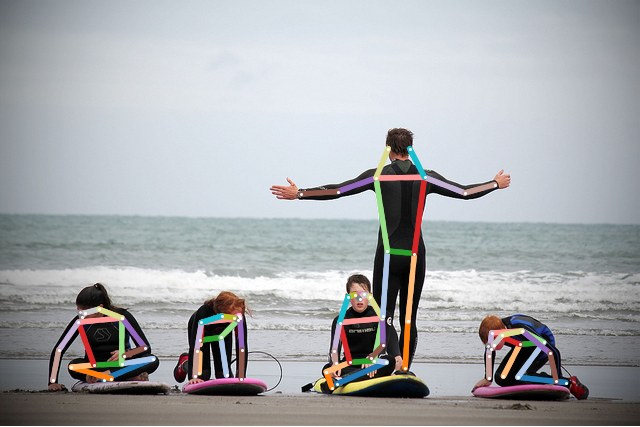
\includegraphics[scale=0.4]{figures/skeleton.png}
    \caption{Example of the human pose estimation using openpifpaf}
    \label{fig:kreiss2019pifpaf}
\end{figure}


\subsection{Neural Network description}
The structure of the neural network that we use in the skeleton based person re-id method can be seen in Figure \ref{fig:skeleton_based_model}. It can be again separated into two parts.

The first part consists of three LSTM layers (see Section \ref{tb:lstm}), each of which is followed by a batch normalization layer. The input to the first LSTM layer is a sequence of 20 34-dimensional vectors representing the $x$ and $y$ coordinates of the 17 most significant joints of the observed body (see previous section). In the last LSTM layer, the whole sequence is combined into one output, that is then fed into the second part of the network.

The second part of the network consists of two Dense layers. The first one has the ReLu activation function, and the second one is the classifying layer and uses the Softmax activation function.

\begin{figure}[h!]
    \centering
    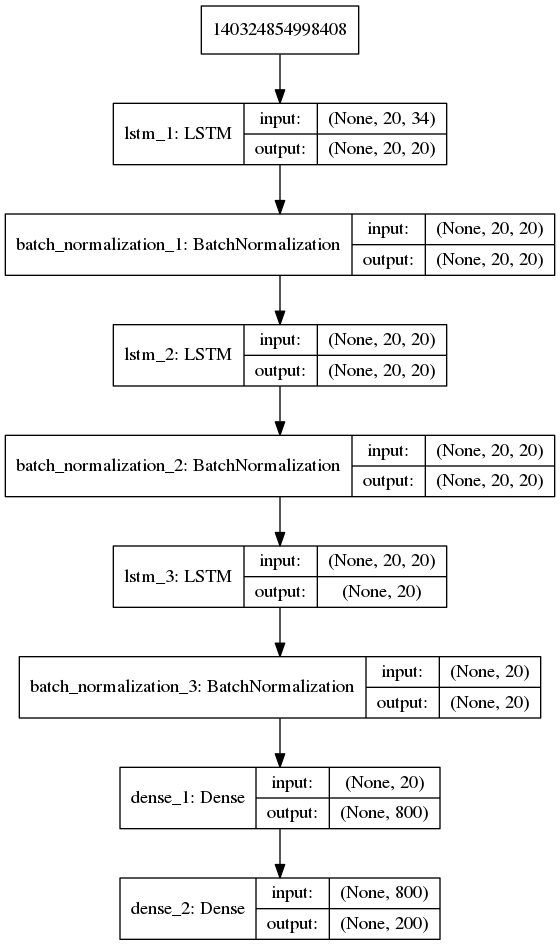
\includegraphics[scale=0.4]{figures/model_kpts.png}
    \caption{Skeleton based model NN}
    \label{fig:skeleton_based_model}
\end{figure}

\section{Combined method}
In the third method, we combine both previous approaches. First, we transform the images into edges. In the second step, we draw the skeleton onto the edges. The model is then provided with sequences of images depicting the edges together with the skeleton. This way, the model itself decides about the relevance of this two information and can combine them accordingly.

\subsection{Combining the edges with skeleton}
At this point, we already have both the edges of the observed identities in the images and the locations of their joints from the previous two methods. In order to depict the skeletons onto the transformed images, what we need to do is to draw lines connecting the adjacent joints. To keep some additional information, we draw the lines depicting hands blue, lines depicting the body green and those highlighting the legs red. An example of a seven-frame sequence with edges and skeleton drawn as described is illustrated in Figure \ref{fig:edges_with_skeleton}.

\begin{figure}[h!]
    \centering
    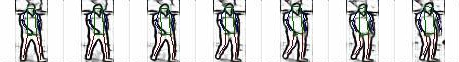
\includegraphics[scale=0.8]{figures/edges_with_skeleton.png}
    \caption{Edges with skeleton example}
    \label{fig:edges_with_skeleton}
\end{figure}

\subsection{Neural Network description}
In the combined method, as the inputs have not changed from the edges method in anything but having the additional skeleton drawn on the video frames, we use the very same neural network as in the edges method (see Figure \ref{fig:nnModel}). 
